% !TEX encoding = UTF-8 Unicode
%%%%%%%%%%%%%%%%%%%%%%%%%%%%%%%%%%%%%%%%%%%%%%%%%%%%%%%%%%%%%%%%%%%%%%%%%%%%%%%%%%%%%%%%%%%%%%%%%%%%%%%%%
%% 
%%  This file is asmejour-template.tex, a template to format papers in the style of ASME journal papers. 
%%
%%  This file is version 1.18 dated 2022/01/10
%%
%%  Author: John H. Lienhard V
%%          Department of Mechanical Engineering
%%          Massachusetts Institute of Technology
%%          Cambridge, MA 02139-4307 USA
%%
%%  Class options include:
%%
%%          * Option to color the vertical bar in the title block [barcolor = colorname] 
%%          *    where colorname is any name def'd by xcolor package; omit barcolor option to get black
%%
%%          * Option to omit the list of figures and list of tables at the end [nolists]
%%
%%          * Math options from M. Sharpe's newtxmath package: upright integrals [upint];
%%          *    [varvw] for a v and w that are better distinguished from Greek nu; [subscriptcorrection]
%%			*	 to fine-tune the placement of math subscripts; and also additional options such as
%%          *    [smallerops, varg, slantedGreek, frenchmath, varbb, cmbraces]. Version 1.6 or higher
%%          *    is recommended.
%%
%%          * Option to include line numbers [lineno]. The lineno package does not number tables, 
%%          *    footnotes, captions, etc. You must run *twice* for proper placement of the numbers. 
%%          *    This option will disable balancing of the column heights on final page.
%%
%%			* Option to balance column heights on final page [balance]. This option sometimes
%%			*    misbehaves, so use it with an awareness that it can create unexpected problems.
%%			*	 This option is not compatible with line numbering.
%%
%%          * Options for copyright notices:
%%			* 	 Omit the ASME copyright from the footer [nocopyright]
%%			*	 Copyright footnote if all authors are government employees  [govt]
%%			*	 Copyright footnote if some authors are government employees [govtsome]
%%			*	 Copyright footnote for government contractors [contractor]
%%
%%          * Option to omit all ASME text fields from the footer [nofoot].
%%
%%			* Options for PDF/A compliance. [pdf-a] will produce PDF/A-3u compliance with sRGB OutputIntent.
%%			*	 [pdfapart= 1 or 2 or 3] and [pdfaconformance= b or u] can enable levels 1b, 2b, 2u, and 3b.
%%			*
%%			*    The most recent versions of LaTeX (2021 and later) are moving toward integrated support for pdf-a, 
%%			*    through \DeclareDocumentMetadata{..}. The asmeconf class supports these new features, which can 
%%			*	 replace the aforementioned class options. (An up-to-date LaTeX installation is required.)
%%
%%          * Many options for calligraphic, script, and fraktur fonts from the mathalfa package; the
%%          *    example value used is: mathalfa=cal=euler (use Euler font for \mathcal)
%%          *    some other options for cal are: dutchcal, zapfc, cm (default), boondox,...
%%          *    frak (fraktur), bb (blackboard bold), scr (script) may also be controlled.
%%
%%          * An option to use newtxtext's superiors font for footnotes [nodefaultsups] and an option
%%          *    for slightly larger small capitals [largesc]
%%
%%          * Options for typewriter font 
%%          *    [hyphenate] allow hyphenation (normally suppressed because for typewriter font is often used for code)
%%			*	 [var0] replace default slashed zero by unslashed zero
%%			*	 [mono] force interword separation to monospacing
%%
%%          * Options for the babel package to support passages in other languages (such as a translated 
%%          *    abstract in an appendix), e.g. [french].  The main language will default to English 
%%          *    unless a different main language is selected, e.g. [main=spanish]. See Appendix C for details.
%%
%%  For details of the newtx and mathalfa packages, refer to their documentation (available at CTAN: http://ctan.org).
%%
%%  The use of commands defined or modified by the asmejour class is illustrated below. In particular, some care
%%  is needed when using complicated math and macros in section headings, to avoid problems with pdf bookmarks, 
%%  as facilitated by the optional argument of \section (also illustrated below).
%%
 %=========================================================
%% 
%% LICENSE: 
%%
%% Copyright (c) 2022 John H. Lienhard
%%
%% Offered under the MIT license: https://ctan.org/license/mit 
%%
%%%%%%%%%%%%%%%%%%%%%%%%%%%%%%%%%%%%%%%%%%%%%%%%%%%%%%%%%%%%%%%%%%%%%%%%%%%%%%%%%%%%%%%%%%%%%%%%%%%%%%%%%

%% Class options are described above.
\documentclass[subscriptcorrection,upint,varvw,barcolor=Goldenrod3,mathalfa=cal=euler,balance,hyphenate,french,pdf-a, nofoot]{asmejour} %


%%%%  pdf metadata  %%%%%%%%%%%%%%%%%%%%%%%%%%%%%%%%%%%%%%%%%%%%%%%%%%%%%%%%%%%%%%%%%%%%%%%%%%%%%%%%%%%

\hypersetup{%
	pdfauthor={Saurav Kambil},                       		   	% <=== change to YOUR name[s]!
	pdftitle={ASME Journal Paper LaTeX Template},                  	% <=== change to YOUR pdf file title
	pdfkeywords={ASME journal paper, LaTeX template, BibTeX style, asmejour class},% <=== change to YOUR pdf keywords
	pdfsubject = {EKF for Robotic Cloth Manipulation},			% <=== change to YOUR subject
%	pdfurl={https://ctan.org/pkg/asmejour},% may delete
	pdflicenseurl={https://ctan.org/pkg/asmejour},% may delete
}

%%%%  Journal name and optional copyright year %%%%%%%%%%%%%%

%% Omit "Journal of". If Journal Name is quite long, use \\ to insert a line break
%<=== change to the name of your journal

%% The default copyright year is the current year
%% \PaperYear{2022} sets 2022; and \PaperYear{} omits the year entirely.
                   
%%%%  end of preamble  %%%%%%%%%%%%%%%%%%%%%%%%%%%%%%%%%%%%%%%%%%%%%%%%%%%%%%%%%%%%%%%%%%%%%%%%%%%%%%%%%
\usepackage{float}
\begin{document}


% Change to your author name[s] and addresses, in the desired order of authors.
% First name, middle initial, last name
% Use title case (upper and lower case letters)
% Note usage below for corresponding author.

\SetAuthorBlock{Saurav Kambil}{Department of Mechanical Engineering,\\
   Carnegie Mellon University,\\
   5000 Forbes Avenue,\\
   Pittsburgh, PA \\
   email: skambil@andrew.cmu.edu} 

% To label one or more corresponding authors put "Name\CorrespondingAuthor". No space after "Name".
% An optional argument can be added if email is not in address block as
%      "Name\CorrespondingAuthor{write@to.me}"
% Can also include multiple emails and use the command more than once for multiple corresponding authors,
%      "Name\CorrespondingAuthor{write@to.him, write@to.her}"

\SetAuthorBlock{Zackory Erickson}{%
Assistant Professor\\
Robotics Institute,\\
Carnegie Mellon University, \\
Pittsburgh, PA \\
email: zackory@cmu.edu
}

%%% Change to your paper title. Can insert line breaks if you wish (otherwise breaks are selected automatically).
\title{Extended Kalman Filter for Real-Time State Estimation of Cloth for Robotic Manipulation }


%%% Change these to your keywords.  Keywords are automatically printed at the end of the abstract.
%%% This command must come BEFORE the end of the abstract.
%%% If you don't want keywords, omit the \keyword{..} command.
\keywords{Extended Kalman Filter, Robotic Cloth Manipulation, Codimensional IPC Model, AprilTags, State Estimation, Dynamic Textile Interaction, Sim-to-Sim Study, Autonomous Fabric Handling, Cloth Dynamics Simulation, Real-Time Robotic Control}

   
%% Abstract should be no more than 250 words
\begin{abstract}
This project explores the application of an Extended Kalman Filter (EKF) to accurately estimate the state of cloth in dynamic manipulation scenarios, a crucial aspect for enhancing the autonomy and efficiency of robotic systems interacting with textile materials. Leveraging the advanced physics simulation capabilities of the codimensional incremental potential contact (IPC) model, the research aims to bridge the gap between virtual simulations and real-world cloth behavior. To achieve a reliable state estimation, the project employs AprilTags—visually recognizable markers—strategically placed across a towel's surface in a mesh-like pattern that mirrors the simulated cloth mesh. This setup facilitates the precise tracking of cloth vertices during gravity drop tests, providing a robust dataset for validating the EKF's performance. A key part of our methodology involves a sim-to-sim study, which rigorously tests the EKF's effectiveness in a controlled simulation environment before real-world application. This study demonstrates that state convergence is achieved within 50 timesteps at a timestep size \(\delta\)\ of 1/240 seconds, showcasing the EKF's capability to quickly adapt and accurately predict the state of the cloth based on the dynamic input data. As the project is in its exploratory phase, the results are preliminary but hold the promise for groundbreaking advancements in the field of dynamic cloth manipulation. This research not only contributes to the foundational understanding of cloth dynamics but also opens new avenues for robotic applications requiring nuanced interaction with flexible materials.
\end{abstract}


\date{\today}%% You can modify this information as desired. 
							%% Putting \date{} will suppress any date.  
							%% If this command is omitted, date defaults to \today
							%% This command must come somewhere before \maketitle

\maketitle %% This command creates the author/title/abstract block. Essential!

%%%%%%%%%%%%%%%%%%%%%%%%%%%%%%%%%%%%%%%%%%%%%%%%%%%%%%%%%%%%%%%%%%%%%%%%%%%%%%%%%%%%%%%%%%%%%%%%%%%%%%%
%%%%%%%%%%%%%%%%%%%%%  End of fields to be completed. Now write! %%%%%%%%%%%%%%%%%%%%%%%%%%%%%%%%%%%%%%

\section{Introduction}

The dynamic manipulation of cloth represents a frontier in the field of robotics, offering profound implications for assistive robotics, industrial automation, and even healthcare\cite{doumanoglou2014autonomous, maitin2010cloth, erickson2018deep, erickson2018tracking, erickson2020assistive, yu2017haptic}. The profound impact of this technology extends beyond mere convenience, potentially transforming the lives of many, especially those requiring assistance with daily tasks. In assistive robotics, the development of autonomous systems capable of manipulating textiles can lead to the creation of robotic assistants that help the elderly or individuals with disabilities dress themselves, enhancing their independence and quality of life.uch innovations could drastically reduce the need for human caregivers for dressing tasks, granting privacy and self-reliance to users.
\begin{figure}
\centering
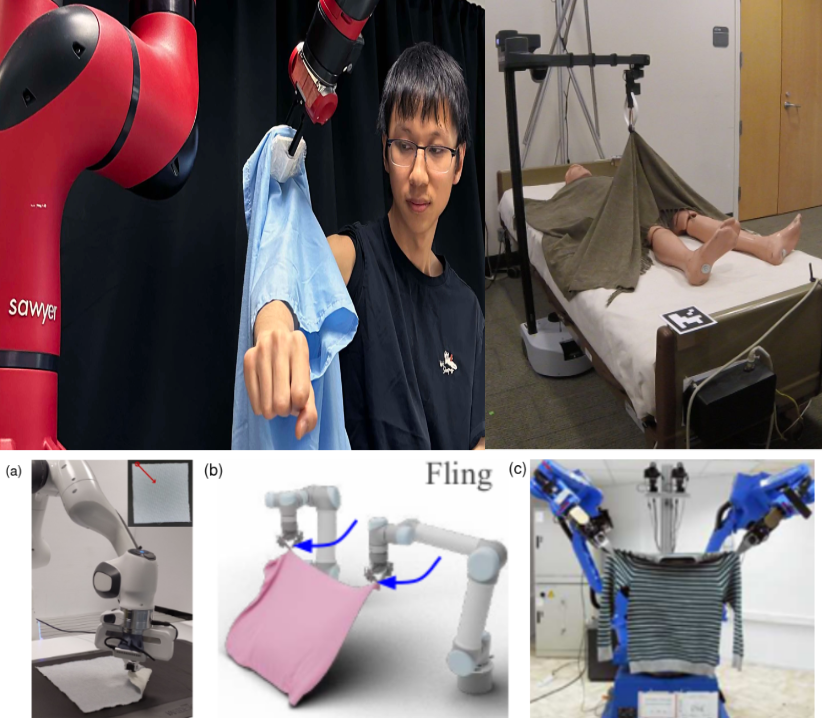
\includegraphics[width=\columnwidth]{CLOTH REPORT PICS/high_level.png}
\caption[Robotic Cloth Manipulation]{(Top left) A robot-assisted dressing system employs a single learned policy to dress various individuals in different poses and garments\cite{Wang2023One}. (Top right) A mobile manipulator, Stretch RE1, applies a policy trained in simulation to uncover a manikin's legs with a blanket\cite{puthuveetil2022bodies}. (Bottom) Demonstrations of action primitives in cloth shaping: (a) Pick-and-Place\cite{lee2021learning}, (b) Pick-and-Fling\cite{ha2022flingbot}, and (c) Gravity-based cloth flattening for efficient manipulation in robotic tasks\cite{doumanoglou2014autonomous}.}
\label{fig:robotic_cloth_manipulation}
\end{figure}

Beyond individual assistance, cloth manipulation robots can play pivotal roles in healthcare environments. They could assist in preparing and folding sterile garments in operating rooms or changing bed linens in hospitals with precision and efficiency, reducing strain on healthcare staff and improving hygiene\cite{seita2019deep}. Bed-making robots, for example, could ensure that hospital beds are always clean and ready for new patients, aiding in infection control by minimizing human contact.

In the industrial sector, cloth manipulation technology heralds a new era of automation in the textile and apparel industries. From cutting fabrics to precise measurements to sewing and quality control, robots equipped with this capability could significantly speed up production lines while maintaining high standards of quality\cite{torgerson1988vision}. They could undertake tasks such as the automatic folding of garments, streamlining the packaging process, or intricate work like embroidery, which requires a high level of precision. This not only boosts productivity but also allows human workers to focus on more complex and less monotonous tasks.

Dynamic robotic cloth manipulation presents profound challenges that stem from its inherent properties and behavior, distinct from those of rigid objects. Cloth is highly deformable, lacking a fixed shape, which means it can bend, fold, and drape in complex, unpredictable ways\cite{borras2020grasping, sanchez2018robotic}. Unlike rigid objects that have well-defined, stable geometries, a piece of cloth can assume an almost infinite number of configurations, each influenced by subtle variations in external forces, interactions with the environment, and its own material characteristics such as weight, stiffness, and texture.

These unique properties of textiles demand that robots not only adapt to the immediate shape and position of the cloth but also anticipate its potential movements in response to manipulative actions. For example, lifting a corner of a blanket might cause other parts to slide or fold unexpectedly, complicating tasks like folding or hanging. Furthermore, the dynamic interaction between different parts of the cloth—such as between layers when folding or wrapping—adds another layer of complexity.

The challenges are exacerbated by the fact that sensing and perception systems in robots, which are typically designed for rigid objects, often struggle to accurately assess and predict the state of cloth. Visual perception can be hindered by the cloth's texture or translucency, and tactile feedback might not provide sufficient information about the cloth's overall configuration\cite{tirumala2022learning}. This results in a need for advanced algorithms and sensory integration to handle the versatile and dynamic nature of cloth manipulation effectively.

This complexity not only affects the physical handling of cloth but also the computational models used to plan and execute tasks. Traditional models of object manipulation are based on rigid-body dynamics, which are ill-suited to describe the behavior of textiles\cite{zheng2024differentiable}. Developing models that can accurately predict the behavior of cloth under various conditions is crucial but remains a significant challenge in the field of robotics. Thus, improving cloth manipulation in robotics involves not only refining the mechanical interaction through innovative gripper designs and manipulation strategies but also enhancing the perception and intelligence of robots to deal with the unpredictable nature of textiles.

Despite its potential, one of the significant hurdles in cloth manipulation is the accurate estimation of the cloth's state — its position, orientation, and deformation — in real-time. Current methods struggle with state estimation due to the high dimensionality of the problem and the limitations of sensory inputs, which often cannot capture the entire state of the cloth precisely. Techniques like vision-based tracking or direct tactile sensing provide partial solutions but often fall short in complex manipulation scenarios due to occlusions, sensor noise, and the computational complexity of modeling cloth physics accurately.

On the other hand, cloth simulation presents a unique challenge in robotics and computer graphics due to the inherently complex behavior of fabric materials. Furthermore, previous works on cloth manipulation or state estimation have largely overlooked the intricacies of cloth physics\cite{clegg2018learning, chen2022efficiently, bertiche2022neural, santesteban2019learning, lahner2018deepwrinkles}. Traditional cloth simulators often struggle to authentically replicate complex fabric deformations, leading to unrealistic simulations that fail to mirror the natural draping and folding of actual materials. Many fall short in handling self-collisions and penetrations that occur with cloth dynamics, resulting in less convincing interactions, especially when the cloth folds or layers upon itself. While interactions between cloth and rigid bodies are commonly well-simulated, the more intricate cloth-to-cloth interactions pose a greater challenge, frequently oversimplified by existing models. Additionally, the computational demands of simulating cloth increase with complexity, and simulators may not scale well, nor accurately represent the diverse material properties of different fabrics, impacting the fidelity of the simulation.



The Codimensional Incremental Potential Contact (C-IPC) model offers a significant leap in cloth simulation, employing a $C^2$ constitutive barrier model for complex deformation dynamics and integrated strain limiting to prevent unrealistic stretching, without inducing the numerical artifacts common in traditional methods\cite{Li2020IPC, Li2021CIPC}. It ensures geometrically accurate interactions by robustly modeling the thickness of codimensional objects, enhancing realism in contact scenarios. C-IPC's innovative additive Continuous Collision Detection (ACCD) method resolves collision with high accuracy, crucial for thin materials, while its unified framework seamlessly simulates different geometric codimensions. Collectively, these features render C-IPC a robust tool for stable simulations across a spectrum of conditions, proving essential for advanced applications in robotics and animation.

This project addresses the aforementioned challenges by exploring the application of an Extended Kalman Filter (EKF) to estimate the state of cloth accurately. EKFs are well-suited for dealing with the non-linear dynamics typical of cloth behavior, offering a robust framework for fusing model predictions with noisy sensory measurements. Leveraging the advanced physics simulation capabilities of the Codimensional Incremental Potential Contact (IPC) model, we aim to bridge the gap between theoretical cloth models and their real-world counterparts]. Furthermore, by employing AprilTags — visually recognizable markers — strategically placed across a towel's surface, we can precisely track specific points on a cloth's surface. This tracking data serves as crucial measurement input for our Extended Kalman Filter (EKF). When combined with our dynamic model, the EKF utilizes this information to produce accurate state estimation.

Our research seeks to fill the gap in dynamic cloth manipulation by enabling more accurate and reliable state estimation, a critical step toward realizing the full potential of robotic systems in interacting with flexible materials. Specifically, this work addresses the question of how the integration of EKFs with physics-based simulation models improve the accuracy of cloth state estimation in dynamic manipulation scenarios.


 



%%%%%%%%%%%%%%%%%%%%%%%%%%%%%%%%%%%%%%%%%%%%%%%%%%%%%%%%%%%%%%%%%%%%%%
\section{Methods}
\subsection{Dynamics Model}
Our study employs the Codimensional Incremental Potential Contact (IPC) physics simulator to model the dynamics of cloth. This simulator is specifically chosen for its exceptional capabilities in handling contact dynamics, which is crucial for accurate simulation of cloth behavior under various manipulation scenarios. By using this advanced simulation framework, we can accurately predict the complex interactions between cloth and its environment, crucial for realistic modeling of textile manipulation tasks.
To fine-tune our model to reflect realistic cloth behaviors, several physical hyperparameters are carefully adjusted:
\begin{itemize}
    \item \textbf{Density of Cloth:} Set to \(100 \, \text{kg/m}^3\), this parameter influences how the cloth interacts with forces such as gravity and aerodynamic drag, affecting its draping and folding behavior.
    \item \textbf{Timestep Size:} The simulation operates with a timestep size (\(\Delta t\)) of \(1/240\) seconds, which allows for temporal alignment to our measurement frames.
    \item \textbf{Young's Modulus:} Set to \(1 \times 10^6 \, \text{Pa}\), this parameter dictates the stiffness of the cloth, impacting how it resists deformation under stress. 
    \item \textbf{Drag Coefficient:} With a value of \(0.01\), this coefficient affects how the cloth interacts with air, modeling the resistance encountered as it moves through its environment.
\end{itemize}

\subsection{Real-Time Simulation Requirements for EKF}

The successful deployment of our Extended Kalman Filter (EKF) for dynamic cloth manipulation hinges crucially on the ability to perform real-time simulations. The real-time criterion is essential as the EKF relies on timely and accurate updates of the cloth's state to predict and correct the system's behavior dynamically. Therefore, the speed of the simulation directly influences the effectiveness of the EKF, necessitating a balance between computational load and temporal accuracy.

To achieve this, we utilized an Nvidia RTX 4090 GPU to simulate a simple cloth mesh under the influence of gravitational forces interacting with a rigid surface. The setup was specifically chosen to emulate realistic cloth behavior such as folding upon impact, presenting a comprehensive test of our simulation framework's capacity to handle complex contact dynamics.

\subsection{Node Count vs Computation Efficiency}
A key variable in our study was the node count, representing discrete points on the cloth mesh where dynamic calculations are performed. A higher node count typically allows for a more detailed simulation of cloth behavior but also increases the computational burden, potentially compromising real-time performance. Our objective was to identify an optimal node count that would support accurate state estimation while maintaining the simulation speed necessary for the EKF to function effectively in real time.

We selected a time step \(\delta\) of 0.01 seconds, balancing the need for accurate simulation with computational efficiency. Performance was evaluated using metrics such as average solver iterations per frame, average time cost per node, and total time per frame, which collectively provided insights into the computational demands of different node counts. These metrics were crucial for determining the maximum node count that could be supported while achieving a frame rate of at least 30 fps, deemed necessary for real-time performance.

\subsection{CPU vs. GPU Performance Evaluation}
An additional aspect of our study involved determining the optimal computational platform for running our simulations, comparing the performance of CPUs and GPUs. Given the parallel processing capabilities of GPUs, they are typically favored for tasks involving high node counts and complex calculations. However, the advantages of GPU parallelization might diminish with fewer nodes, where the workload might be better suited for the high-powered cores of CPUs. To objectively assess which platform—CPU or GPU—delivers better performance for our specific simulation needs, we conducted comparative tests using both an Intel i9 12900 CPU and an Nvidia RTX 4090 GPU. The results of these tests are crucial for deciding the most efficient computing resource, considering factors such as node count, simulation speed, and real-time performance requirements.



\subsection{State Measurement}
To accurately measure the state of the cloth, we incorporate AprilTags in a mesh-like configuration embedded within the cloth structure. These tags are visual markers designed to be easily recognizable and are used here to precisely track the movement and deformation of the cloth in real-time. The cloth in our experiments as shown in fig. 2 is outfitted with a mesh consisting of 168 tags that correspond directly to the nodes within the IPC simulator. We use two GoPro cameras strategically positioned to capture all tags from multiple angles, thus minimizing occlusions and ensuring comprehensive coverage of the cloth's surface during manipulation.
% Inserting a single-column figure
\begin{figure}[ht]
\centering
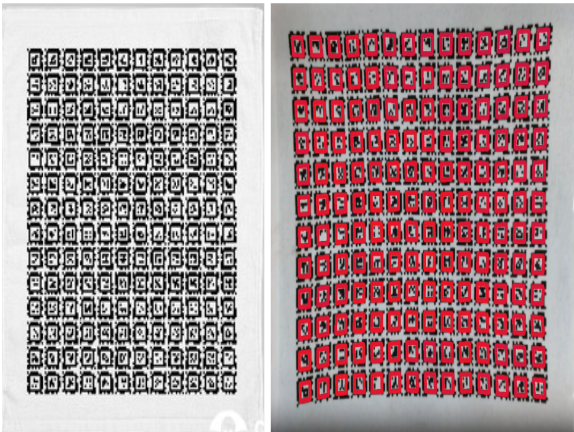
\includegraphics[width=\linewidth]{CLOTH REPORT PICS/Tags.png} % Adjust the image path and extension
\caption{Left- A grid of 168 AprilTags affixed to a cloth for accurate 3D position measurement. Right - The same cloth with detected AprilTags annotated in red by the camera measurement system.}
\label{fig:yourlabel}
\end{figure}


\subsection{Experimental Setup}
Our experimental setup as shown in Fig. 3 comprises an aluminum T-slot frame engineered for consistent and repeatable drop tests of cloth samples. The cloth is affixed by its four corners onto the frame, with two adjacent corners designed to release simultaneously to initiate the drop. This mechanism simulates the cloth's free-falling motion, allowing us to observe the dynamic behavior of the cloth under gravity's influence, simulating a realistic scenario that might be encountered in everyday tasks such as laundry handling or bed-making. The simulation incorporates a total of 238 nodes, with the additional nodes on the cloth's boundaries providing finer detail on edge interactions, which are not directly observable by our cameras.
\begin{figure}[H]
\centering
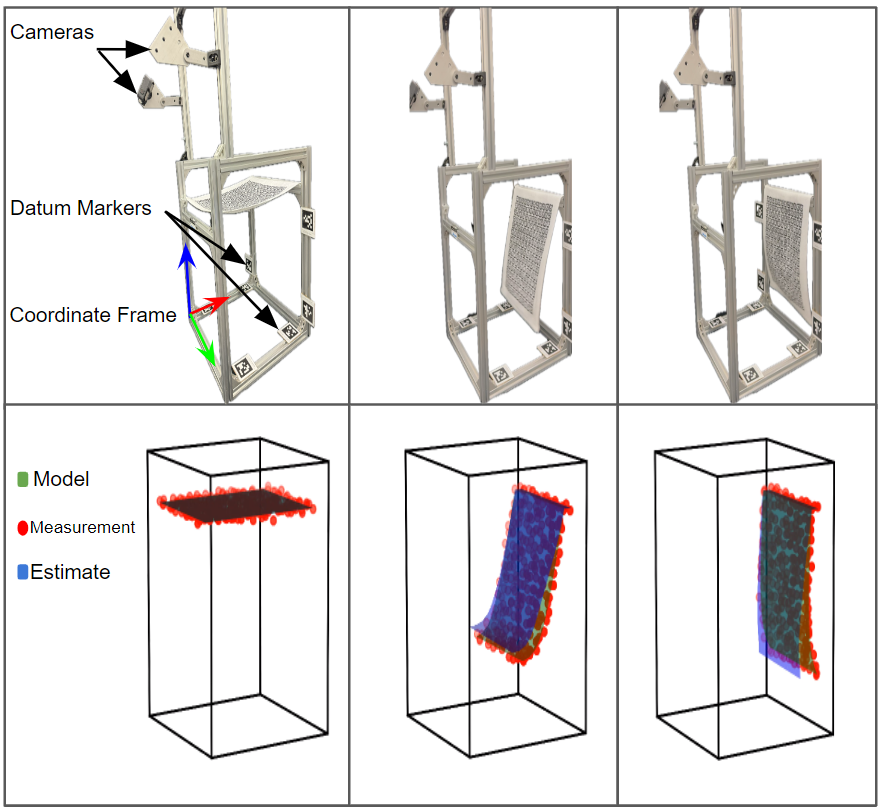
\includegraphics[width=\linewidth]{CLOTH REPORT PICS/Setup.png} % Adjust the image path and extension
\caption{Experimental setup for dynamic cloth manipulation studies. Top: The aluminum T-slot frame holding the cloth at four corners, with two corners released simultaneously to initiate the drop test. Datum markers and a coordinate frame are indicated for spatial reference. GoPro cameras are positioned to capture the cloth's motion from multiple angles. Bottom: Corresponding simulation visuals illustrating the cloth's model (green), the measurement data (red), and the simulation estimate (blue), providing a comparative analysis between the experimental setup and the sim2sim environment}
\label{fig:yourlabel}
\end{figure}


The motion of the cloth during the drop test is meticulously captured using a pair of strategically positioned GoPro cameras. These high-speed cameras are angled to encompass the entire trajectory of the cloth, ensuring comprehensive coverage of the cloth's sweeping motion. Additional AprilTags are placed at known locations on the frame to facilitate the accurate capture of the camera coordinate frames, critical for the post-processing and alignment of the captured data with the simulation models.


\subsection{State Estimation}
For state estimation, our methodology employs the Extended Kalman Filter (EKF), specifically utilizing its Joseph form. The Joseph form is particularly beneficial for its numerical stability and the ability to maintain the symmetry and positive definiteness of the covariance matrix, which are crucial for the high-dimensional state estimation involved in cloth simulation. This form of EKF is adept at handling the non-linear dynamics characteristic of cloth materials, ensuring that our state estimation remains robust even in the face of uncertain and highly variable cloth behaviors.

The EKF is chosen for its proven effectiveness in integrating noisy measurements from our camera system with predictions based on the Incremental Potential Contact (IPC) model. By obtaining the Jacobians of the model from CIPC directly, the EKF facilitates fast state estimation, which is indispensable for real-time applications. This efficiency stands in stark contrast to methods like the Unscented Kalman Filter (UKF), which would require running the simulation 477 times per frame for our scenario, considering we monitor the positions and velocities of 238 nodes. Such a computational load is infeasible for our real-time requirements, highlighting why the EKF's requirement for only the mean and covariance of the state predictions presents a significant advantage.

Additionally, the EKF approach is instrumental in refining the accuracy and reliability of our state estimation. By tracking both the positions and velocities of all nodes within the simulator, we are able to capture a comprehensive picture of the cloth's dynamics. Our state representation is detailed, accounting for the complex interactions and the evolution of the cloth's behavior over time, which is pivotal for the successful manipulation and control of the cloth in various applications.

\subsection*{Noise Parameters}
The noise parameters configured in the EKF are crucial for tuning the filter to the specific characteristics of our simulation:
\begin{itemize}
    \item \textbf{Process Variance:}
    \begin{itemize}
        \item Position process variance: \( \sigma^2_{\text{position}} = 0.001^2 \)
        \item Velocity process variance: \( \sigma^2_{\text{velocity}} = 0.01^2 \)
    \end{itemize}
    \item \textbf{Measurement Variance:}
    \begin{itemize}
        \item \( \sigma^2_{\text{measurement}} = 0.005^2 \)
    \end{itemize}
    \item \textbf{Initial State Error Variance:}
    \begin{itemize}
        \item Initial position error variance: \( \sigma^2_{\text{initial position}} = 0.1^2 \)
        \item Initial velocity error variance: \( \sigma^2_{\text{initial velocity}} = 1.0^2 \)
    \end{itemize}
\end{itemize}

\subsection{Validation}
Initial validation of our methodology is conducted through a simulation-to-simulation (sim2sim) test. Here, a second, deliberately noisier version of the IPC simulator mimics real-world sensor noise and environmental factors, serving as a pseudo-real environment to test the EKF's performance. This step is critical for understanding the robustness of our approach under less ideal and more variable conditions before proceeding to real-world testing.
The simulation as shown in Fig.2 showcases the cloth's modeled behavior (represented in green), the raw measurement data captured by the cameras (in red), and our simulation's estimation of the cloth's state (in blue). This tripartite visualization enables a detailed comparison and validation process, ensuring that our simulation models are accurately reflecting the physical dynamics observed during the experimental drop tests.

We analyze the performance of the EKF by examining the convergence of the covariance matrices and the containment of the innovation vector within three standard deviations \(3\sigma\), confirming the filter's operational validity.


%%%%%%%%%%%%%%%%%%%%%%%%%%%%%%%%%%%%%%%%%%%%%%%%%%%%%%%%%%%%%%%%%%%%%%%%%%%%%%%
\section{Results}
\subsection{Real Time Simulation Capablities}
In this investigation, we specifically aimed to identify the maximum number of states that our simulation can handle while still operating in real time, to ensure efficient state estimation for cloth dynamics. The evaluation was conducted using an Nvidia RTX 4090 GPU. We simulated a simple cloth mesh undergoing gravitational forces and interacting with a rigid surface, which required the mesh to fold upon impact. This scenario, while straightforward, presented a rigorous challenge due to the intricate contact dynamics and the cloth's tendency to fold, offering a robust test for our simulation framework.

The evaluation metrics included average solver iterations, which reflect the Newton steps needed for the simulation to converge, as well as the average time cost per node, and the cumulative time per frame. These simulations were run with a time step \(\delta\) of 0.01 seconds, a parameter selected to ensure a reasonable balance between simulation accuracy and performance. We translated the time per frame into frames per second (fps) and used a threshold of approximately 30 fps to define real-time performance.

The results, summarized in Table 1, demonstrate that our simulation can achieve real-time performance with a node count in the low hundreds, which aligns with our objectives for efficient and accurate state estimation. The findings have been instrumental in optimizing our Extended Kalman Filter (EKF) framework, and based on this study, we have chosen to implement 238 nodes in our simulation for the cloth model, as this node count allows us to maintain a real-time update rate, a crucial factor for potential real-world applications in dynamic cloth manipulation.
\begin{table*}[!htbp]
\centering
\caption{Performance evaluation of the GPU-accelerated IPC simulation for real-time state estimation. The tests were conducted on an Nvidia RTX 4090, with a simulation time step (\(\Delta t\)) of 0.01 seconds.}
\label{tab:gpu_performance}
\begin{tabular}{|c|c|c|c|c|c|}
\hline
\textbf{Nodes} & \textbf{Avg. Time Cost (ms)} & \textbf{Avg. Solver Iterations} & \textbf{Time per Frame (ms)} & \textbf{Frames per Second} & \textbf{Log(Nodes)} \\ \hline
1       & 4.7   & 2  & 9     & 106.38 & 0 \\ \hline
100     & 7.0   & 6  & 42    & 23.81  & 2 \\ \hline
1000    & 10.4  & 20 & 208   & 4.81   & 3 \\ \hline
10000   & 17.5  & 45 & 788   & 1.27   & 4 \\ \hline
200000  & 19.0  & 45 & 855   & 1.17   & 5.3 \\ \hline
\end{tabular}
\end{table*}

\subsection{CPU vs GPU Computation}

 Another pivotal decision is the selection between utilizing the CPU or GPU for our IPC simulations. Given that GPUs are typically favored for their parallel processing capabilities, it would be a common presumption that they would consistently outperform CPUs; this, however, is not always the case. The advantage of GPU parallelization diminishes with smaller node counts, where the simulation tasks are less numerous and less amenable to parallel execution. On the other hand, CPUs, with a smaller number of high-powered cores, may excel in handling simulations with fewer nodes where task parallelization is less critical.

To objectively evaluate the performance trade-offs between CPU and GPU, we conducted a thorough investigation to compare the frames per second (fps) attainable by an Intel i9 12900 CPU and an RTX 4090 GPU across a spectrum of node counts. The results of this study are presented in Table 2. Notably, at a node count of 100, which is proximate to our operational target for real-time state estimation, the CPU demonstrated superior performance over the GPU, suggesting that the high computational capabilities of the CPU cores are more effectively utilized in simulations of this scale.

Thus, despite the general trend towards GPU utilization in computational tasks, our specific requirement of simulating approximately 100 nodes for accurate cloth dynamics places us in a unique scenario where the CPU is not only sufficient but preferable. This is further affirmed by the observed data, indicating that the CPU maintains an edge in fps output at this node count. As a result, for our intended cloth model with 238 nodes, where real-time performance is essential, we have determined that the CPU version of our IPC simulator is the optimal choice, ensuring both the necessary speed and computational efficiency for our tasks.


\begin{table}[ht]
\centering
\caption{Performance comparison between CPU (Intel i9 12900) and GPU (RTX 4090) for IPC simulations, showcasing the relative efficiency at various node counts.}
\label{tab:ipc_performance_comparison}
\begin{tabular}{|c|c|c|}
\hline
\textbf{\#verts} & \textbf{CPU fps (Intel i9 12900)} & \textbf{GPU fps (RTX 4090)} \\ \hline
9       & 289   & 120 \\ \hline
100     & 69.6  & 40  \\ \hline
1024    & 5.217 & 7.5 \\ \hline
4225    & 0.878 & 3.8 \\ \hline
200000  & NA     & 1.8 \\ \hline
\end{tabular}
\end{table}

\subsection{Sim2Sim Study}

We evaluated our Extended Kalman Filter (EKF) implementation through a simulation-to-simulation study, aimed at estimating the state of cloth in a gravity drop test scenario. This assessment was designed to address the challenge of state observability and covariance divergence inherent in our EKF model when adapting from a simulator environment to a real-world setup. Three distinct measurement cases were considered:

\begin{itemize}
    \item \textbf{Full State Measurement:} This method incorporates both the position and velocity data of all nodes.
    \item \textbf{Partial State Measurement:} This approach includes only the position data of all nodes.
    \item \textbf{Restricted State Measurement:} This method is limited to position data from nodes that correspond to real-world tags.
\end{itemize}

The results depicted in the innovation evolution graphs in Fig. 4 indicate a stable behavior of measurement updates across time, with a controlled variance that suggests a consistent performance of the Extended Kalman Filter (EKF) in assimilating measurements with the model predictions. The innovation, which is the difference between the actual measurements and the predictions, remains within a bounded range, signifying that the EKF is correctly tuned to handle the non-linear dynamics of the cloth simulation.

Moreover, the covariance evolution charts in Fig. 5 offer insights into the EKF's estimation certainty. Initially high covariance values, which indicate greater uncertainty, gradually stabilize as the filter processes more data over time. This stabilization reflects the EKF's ability to converge towards a more confident state estimation as it assimilates more information about the system's dynamics.

Comparing the results between systems with different node counts (168 vs. 238) reveals the impact of the number of states on the performance of the state estimation process. The system with 238 nodes demonstrates a slightly higher level of noise in the innovation plots, which could be attributed to the increased complexity and higher dimensional state space being estimated.

The results, depicted in Fig. 6, illustrate the innovation vector for each scenario within the bounds of the expected 3-sigma position covariance range. This consistency across all three cases demonstrates the robustness of our EKF in maintaining bounded innovation despite varying levels of measurement comprehensiveness.


% % Inserting a single-column figure
% \begin{figure}[ht]
% \centering
% 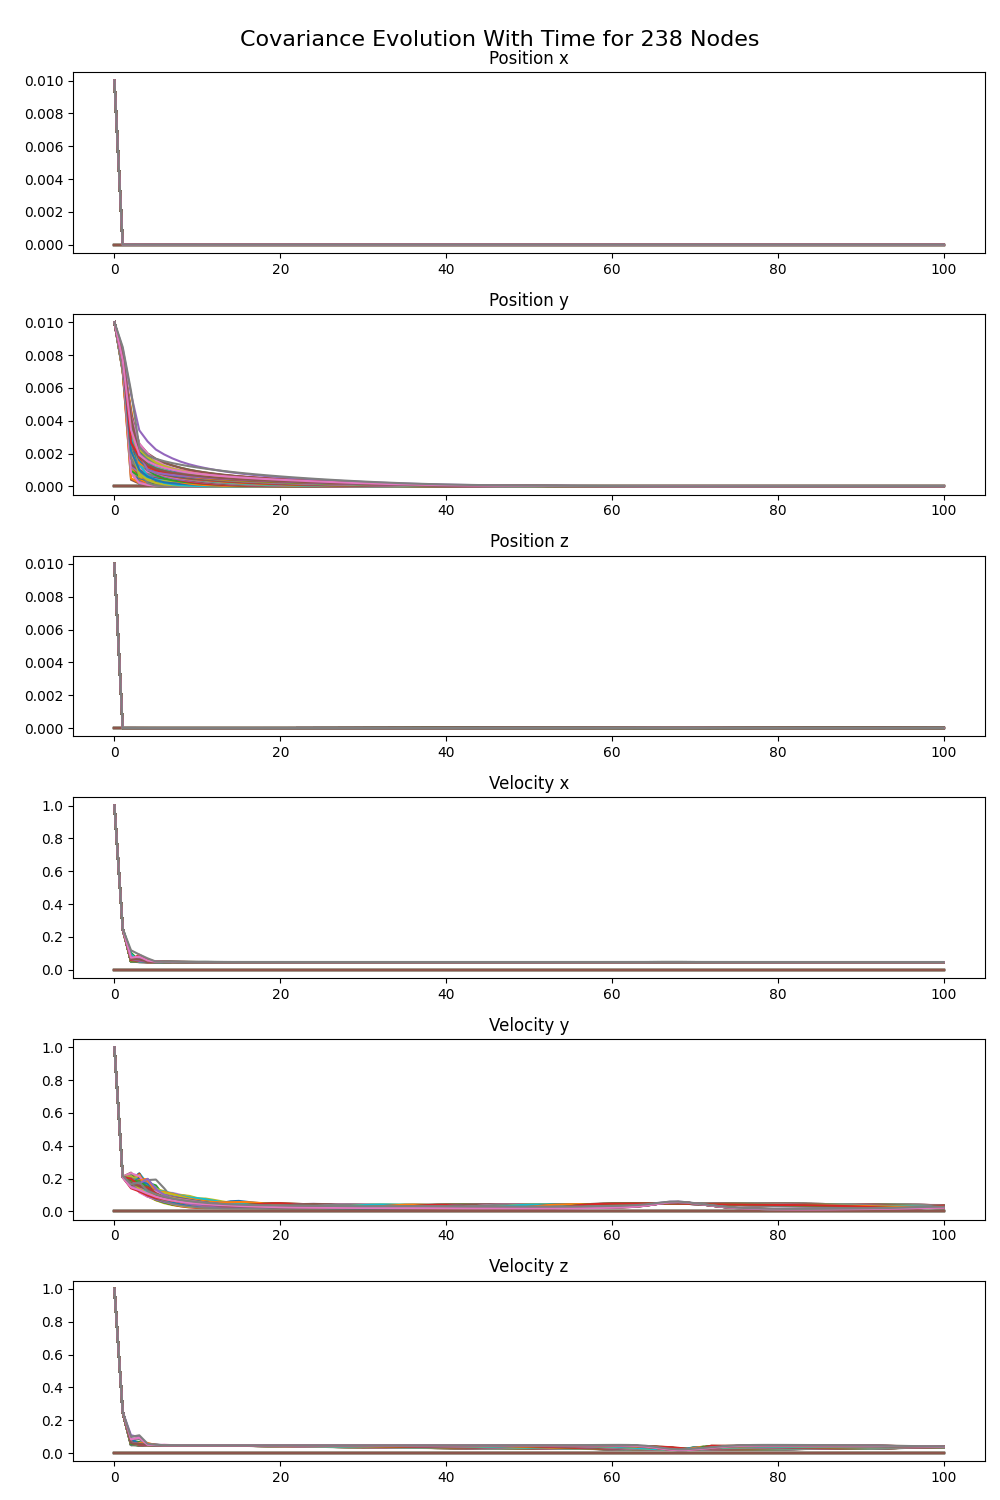
\includegraphics[width=\linewidth]{CLOTH REPORT PICS/covariance 238.jpg} % Adjust the image path and extension
% \caption{Evolution of covariance values for position and velocity states of 238 nodes for full-state system, showcasing the variability in estimation confidence through time.}
% \label{fig:yourlabel}
% \end{figure}

% % Inserting a single-column figure
% \begin{figure}[ht]
% \centering
% 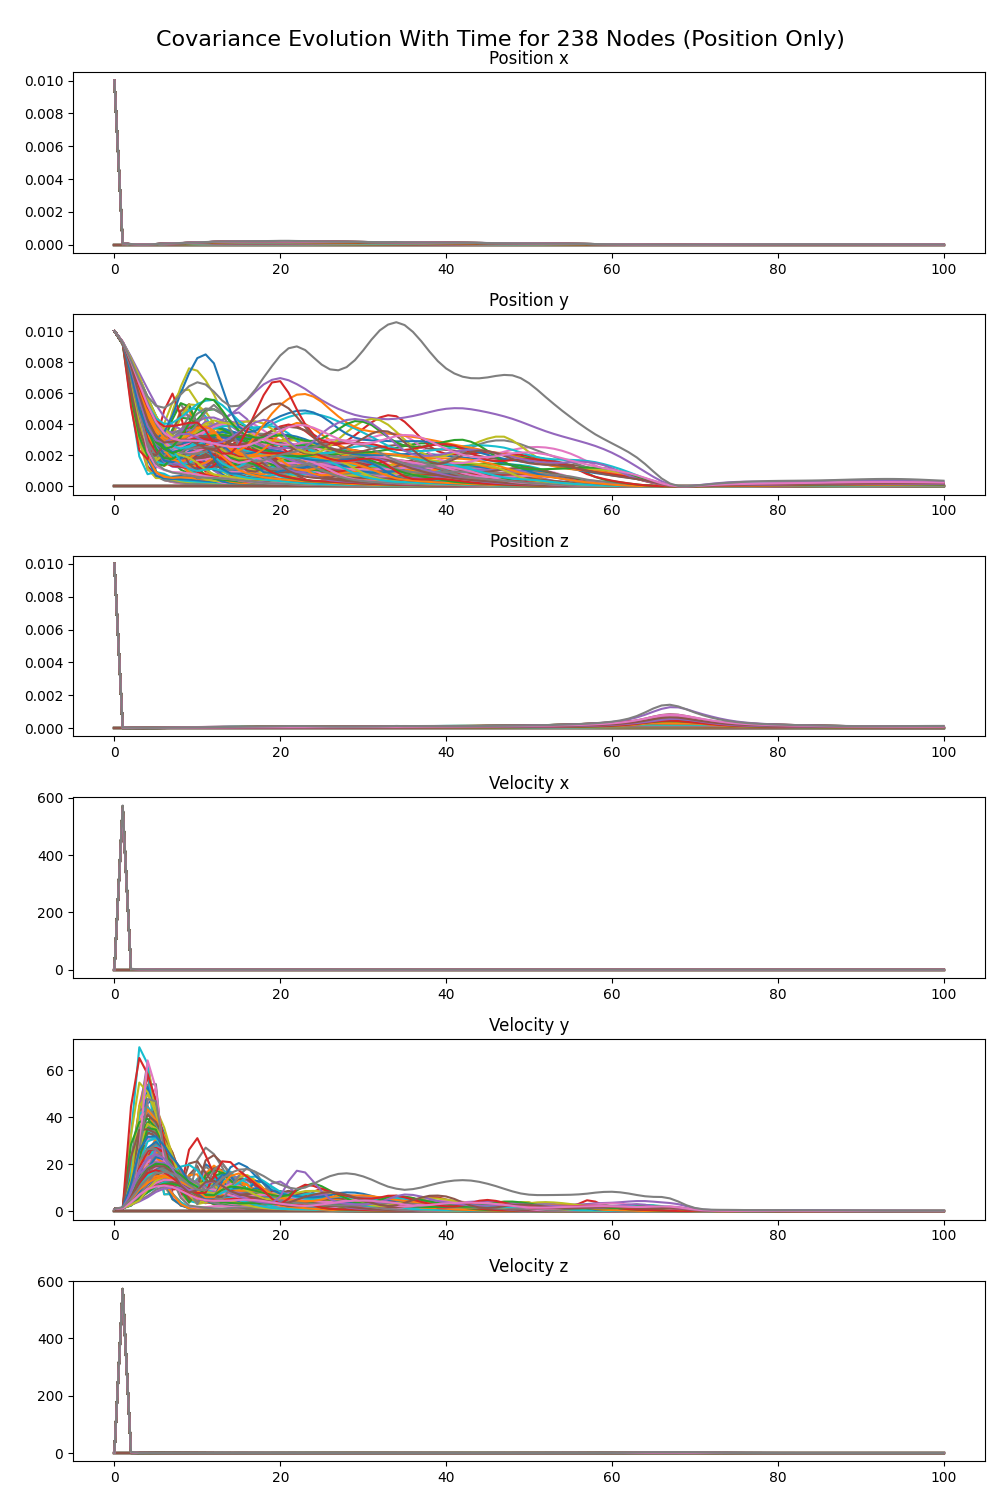
\includegraphics[width=\linewidth]{CLOTH REPORT PICS/covariance 238 p.jpg} % Adjust the image path and extension
% \caption{Evolution of covariance values for position and velocity states of 238 nodes, showcasing the variability in estimation confidence through time}
% \label{fig:yourlabel}
% \end{figure}

% % Inserting a single-column figure
% \begin{figure}[ht]
% \centering
% 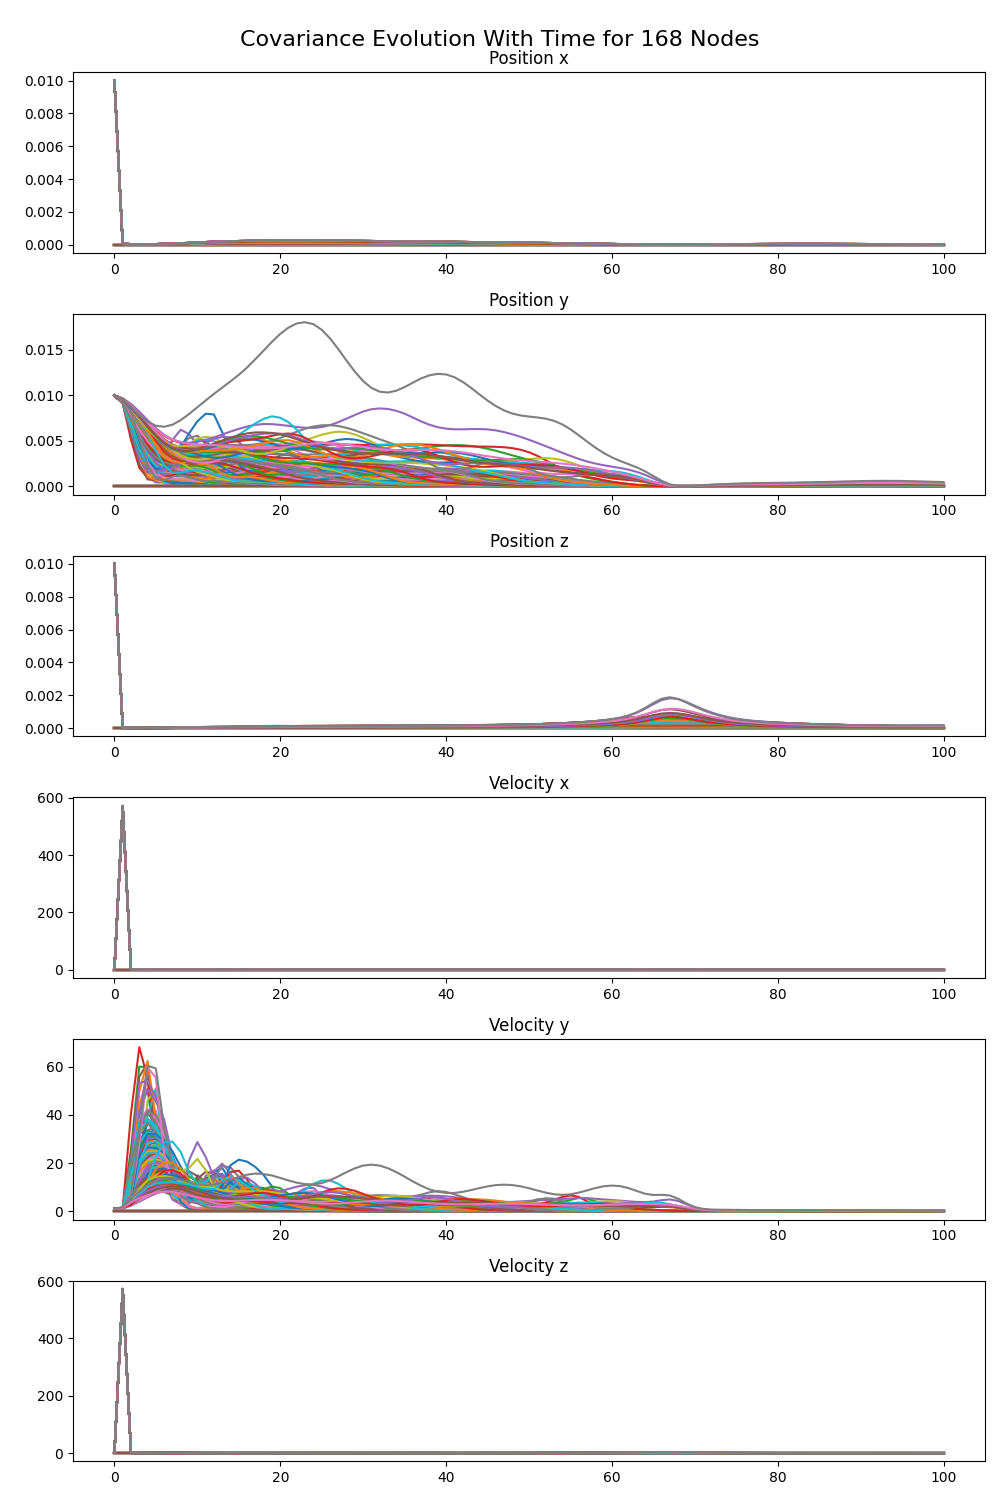
\includegraphics[width=\linewidth]{CLOTH REPORT PICS/covariance 168.jpg} % Adjust the image path and extension
% \caption{Evolution of covariance values for position and velocity states of 168 nodes, showcasing the variability in estimation confidence through time}
% \label{fig:yourlabel}
% \end{figure}
\begin{figure*}[ht]
    \centering
    \begin{subfigure}[b]{0.32\linewidth}
        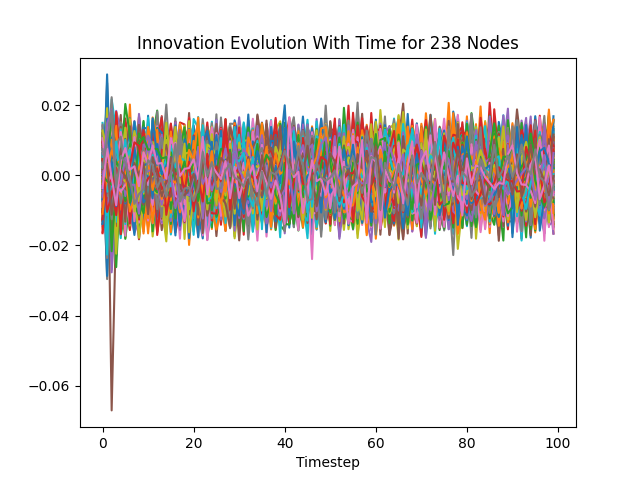
\includegraphics[width=\linewidth]{CLOTH REPORT PICS/innovation 238.jpg}
        \caption{238 nodes, full-state system,}
        \label{fig:innovation-238-full}
    \end{subfigure}
    \hfill % optional: add horizontal space between figures
    \begin{subfigure}[b]{0.32\linewidth}
        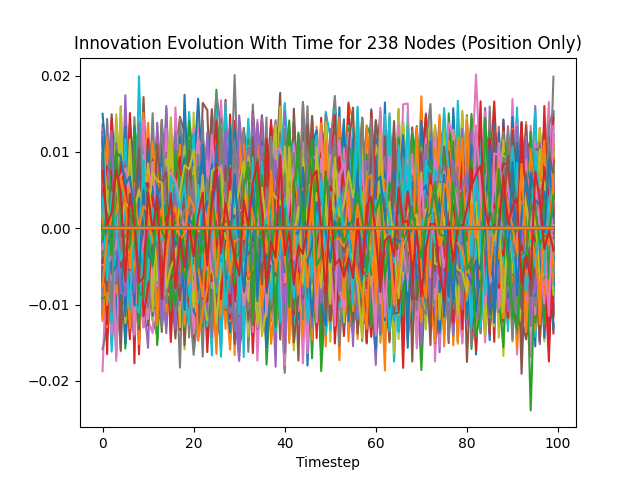
\includegraphics[width=\linewidth]{CLOTH REPORT PICS/innovation 238p.jpg}
        \caption{238 nodes, position only}
        \label{fig:innovation-238-pos}
    \end{subfigure}
    \hfill % optional: add horizontal space between figures
    \begin{subfigure}[b]{0.32\linewidth}
        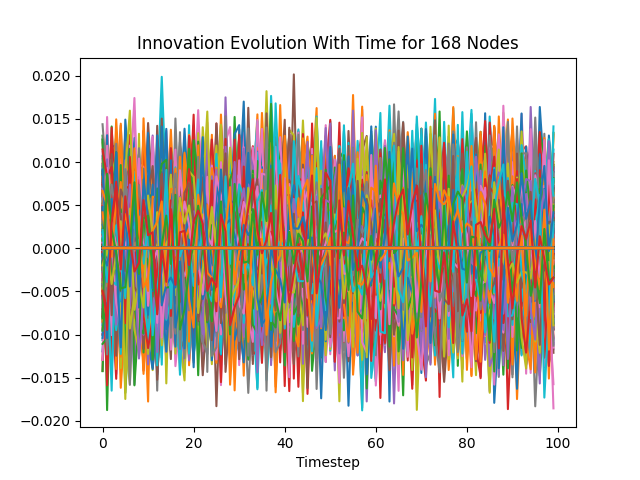
\includegraphics[width=\linewidth]{CLOTH REPORT PICS/innovation 168.jpg}
        \caption{168 nodes, position only}
        \label{fig:innovation-168}
    \end{subfigure}
    \caption{Innovation evolution for position and velocity states of cloth nodes over time, illustrating the variance in measurement updates relative to the predicted state estimates across different configurations.}
    \label{fig:innovations}
\end{figure*}
\begin{figure*}[ht]
    \centering
    \begin{subfigure}[b]{0.32\linewidth}
        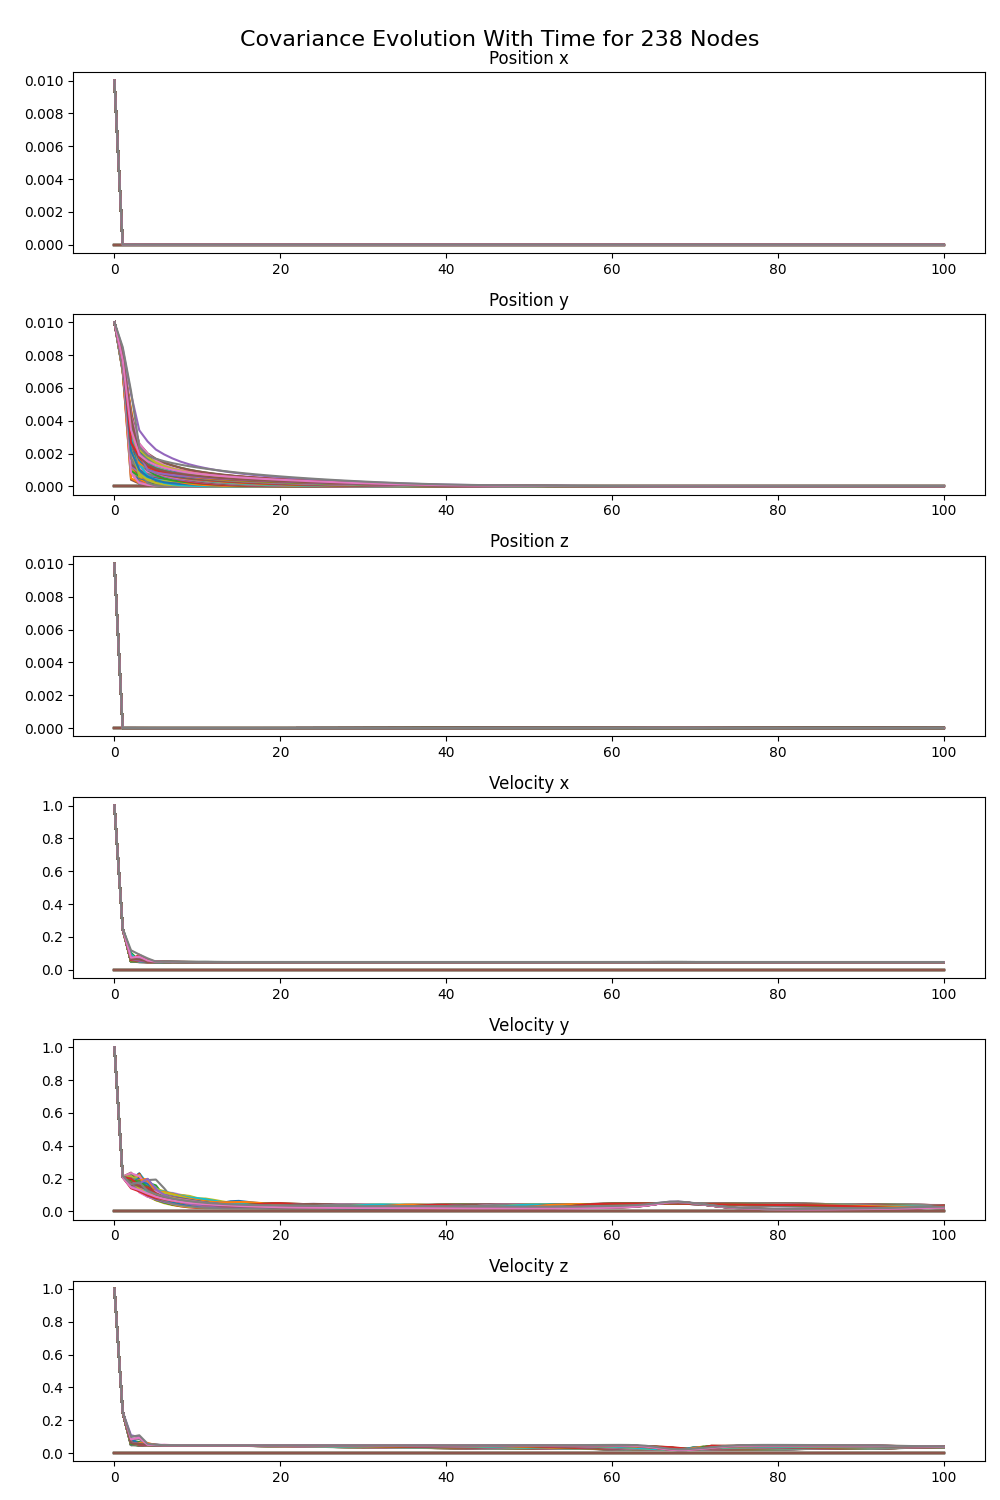
\includegraphics[width=\linewidth]{CLOTH REPORT PICS/covariance 238.jpg}
        \caption{238 nodes, full state}
        \label{fig:covariance-238-full}
    \end{subfigure}
    \hfill % optional: add horizontal space between figures
    \begin{subfigure}[b]{0.32\linewidth}
        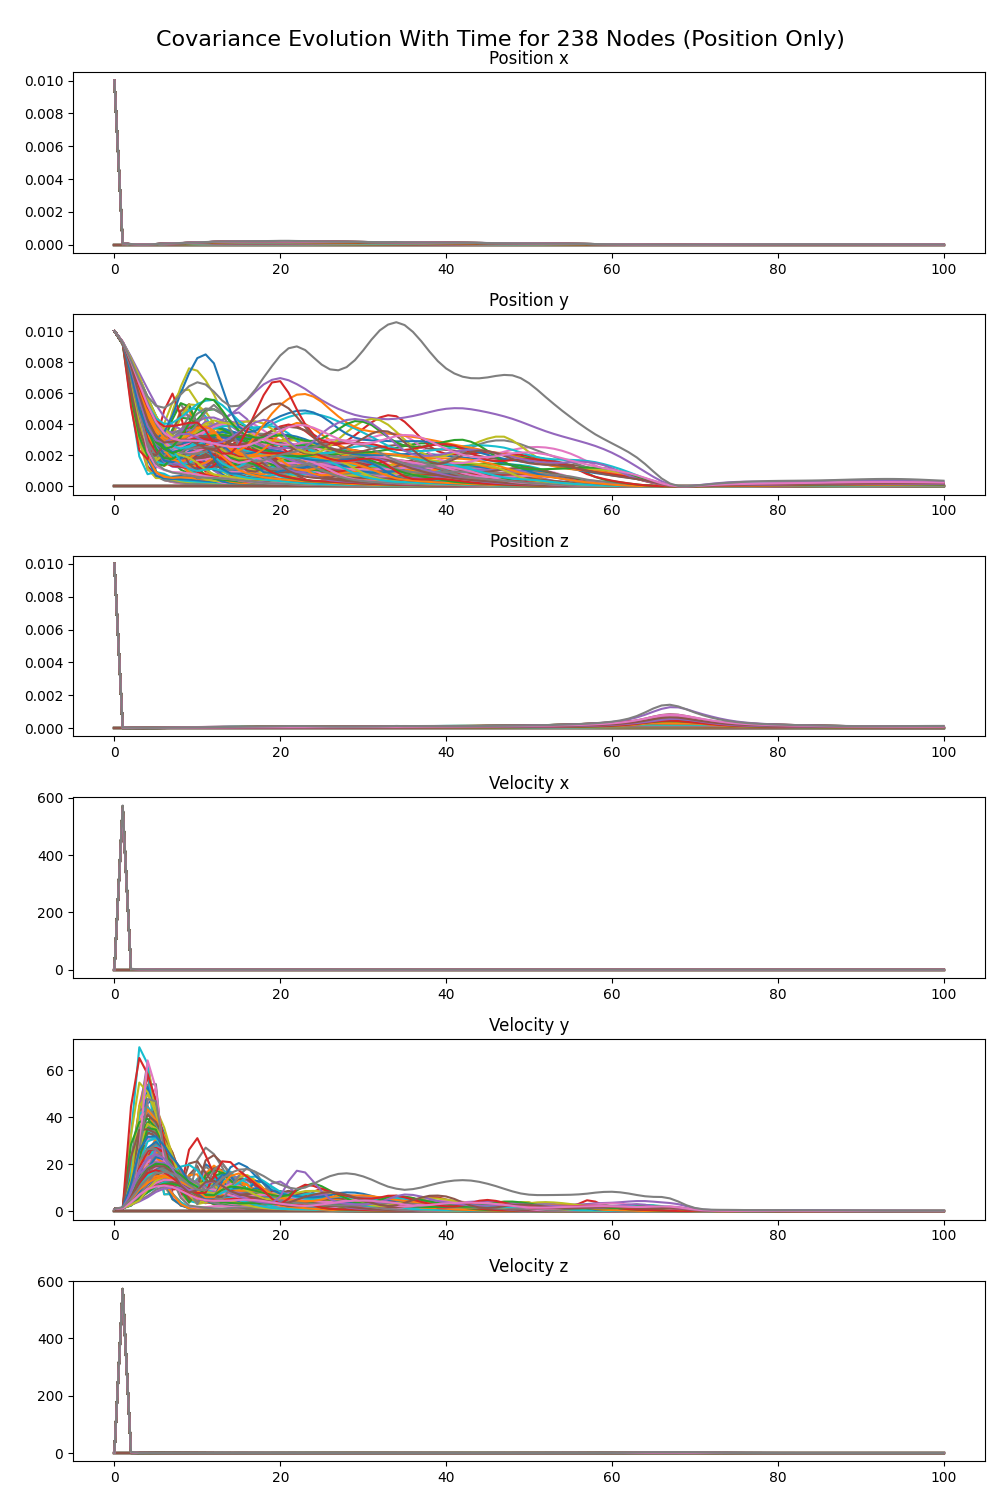
\includegraphics[width=\linewidth]{CLOTH REPORT PICS/covariance 238 p.jpg}
        \caption{238 nodes, position only}
        \label{fig:covariance-238-pos}
    \end{subfigure}
    \hfill % optional: add horizontal space between figures
    \begin{subfigure}[b]{0.32\linewidth}
        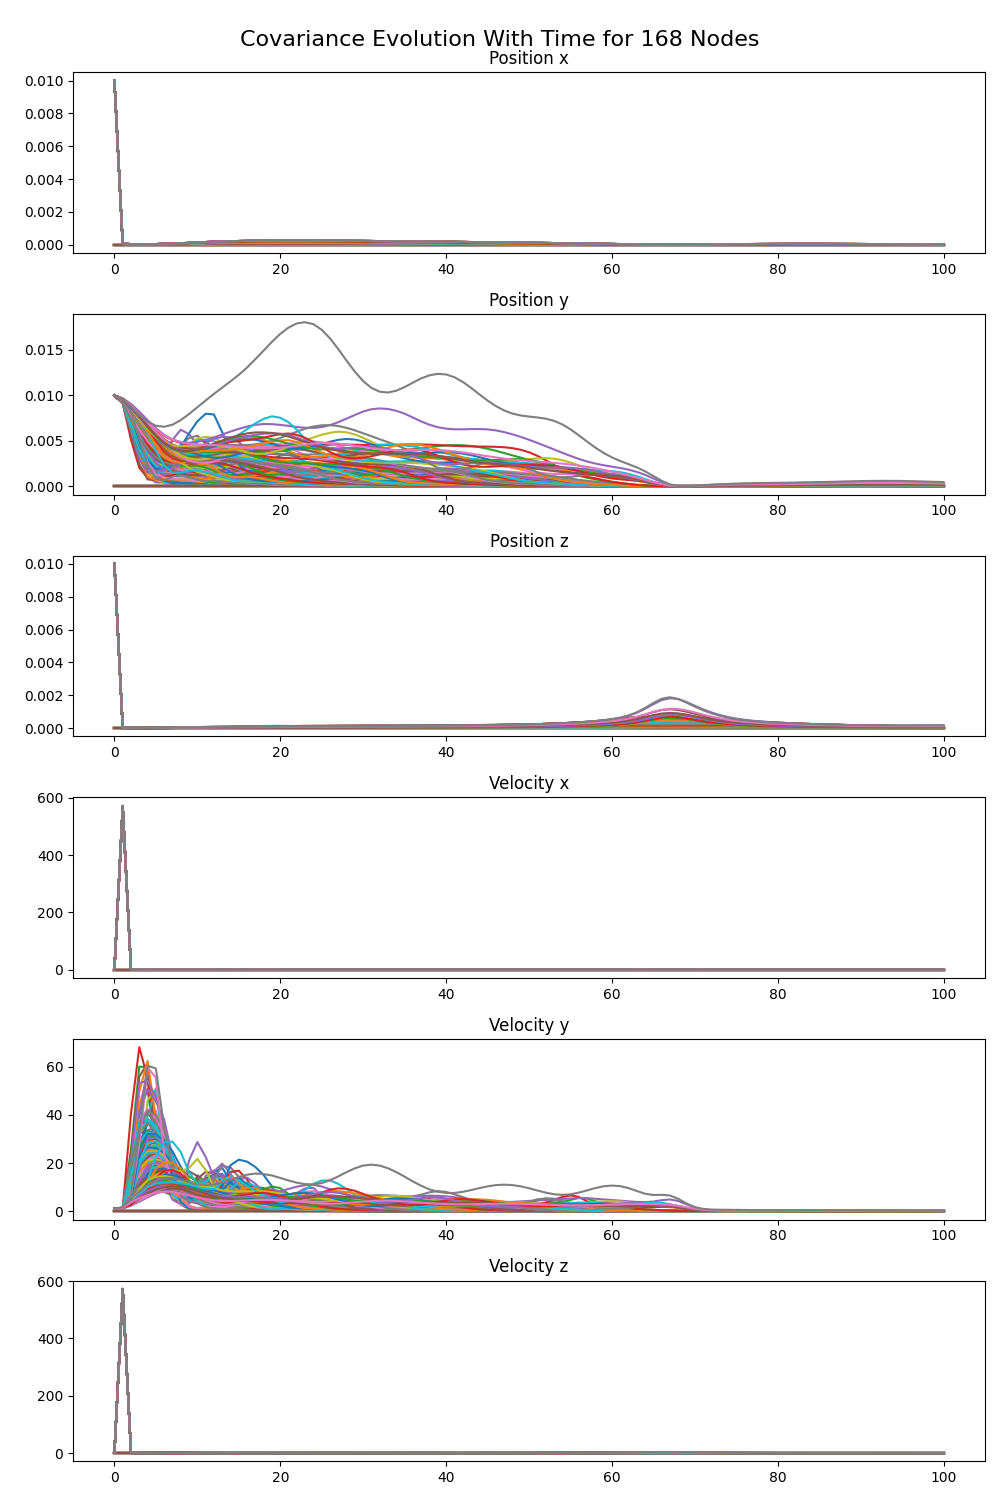
\includegraphics[width=\linewidth]{CLOTH REPORT PICS/covariance 168.jpg}
        \caption{168 nodes, position only}
        \label{fig:covariance-168}
    \end{subfigure}
    \caption{Evolution of covariance values for position and velocity states of cloth nodes in a dynamic manipulation scenario, showcasing the variability in estimation confidence over time for different node configurations and measurement setups.}
    \label{fig:covariances}
\end{figure*}

% % Inserting a single-column figure
% \begin{figure}[ht]
% \centering
% 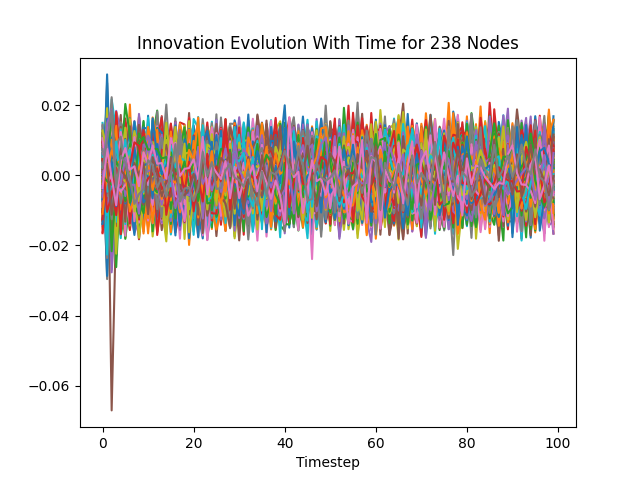
\includegraphics[width=\linewidth]{CLOTH REPORT PICS/innovation 238.jpg} % Adjust the image path and extension
% \caption{Innovation evolution for full-state system of 238 nodes over time, displaying the variance in measurement updates relative to the predicted state estimates.}
% \label{fig:yourlabel}
% \end{figure}

% % Inserting a single-column figure
% \begin{figure}[ht]
% \centering
% 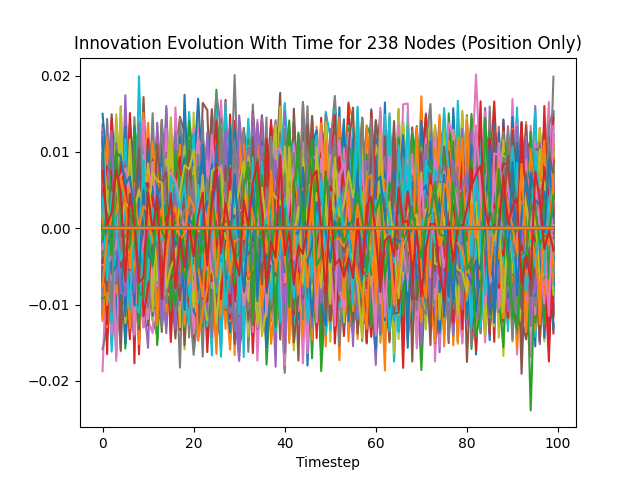
\includegraphics[width=\linewidth]{CLOTH REPORT PICS/innovation 238p.jpg} % Adjust the image path and extension
% \caption{Innovation evolution for position states of 238 nodes over time, displaying the variance in measurement updates relative to the predicted state estimates.}
% \label{fig:yourlabel}
% \end{figure}

% % Inserting a single-column figure
% \begin{figure}[ht]
% \centering
% 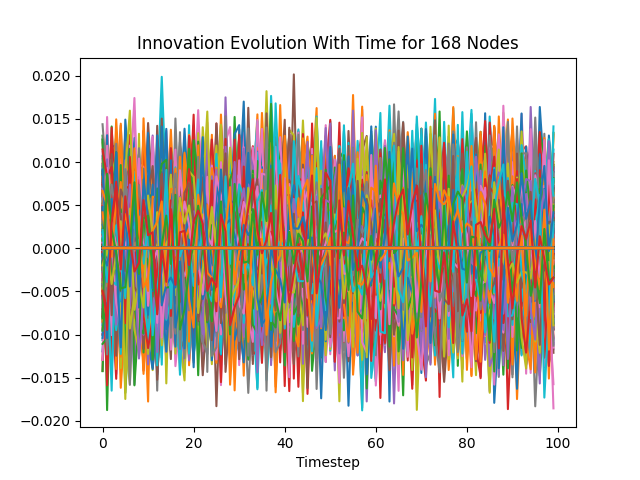
\includegraphics[width=\linewidth]{CLOTH REPORT PICS/innovation 168.jpg} % Adjust the image path and extension
% \caption{Innovation evolution for position states of 168 nodes over time, displaying the variance in measurement updates relative to the predicted state estimates.}
% \label{fig:yourlabel}
% \end{figure}


% Inserting a two-column figure
\begin{figure*}[t]
\centering
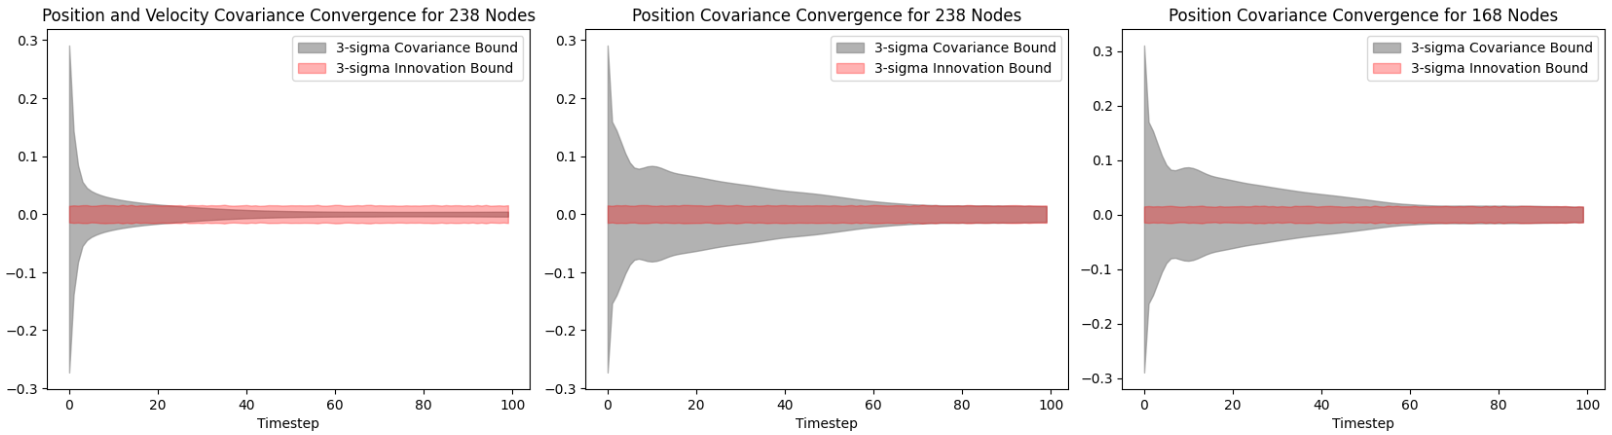
\includegraphics[width=\textwidth]{Covariance Bound.png} % Adjust the image path and extension
\caption{Evaluation of Innovation Vector Boundedness in EKF State Estimation for Cloth Dynamics Across Different Measurement Scenarios. Panel (1) demonstrates the EKF's innovation for all state measurements (positions and velocities) across all nodes, revealing a tightly bounded innovation sequence within the 3-sigma position covariance range. Panel (2) depicts the scenario where only node positions are measured, showing a similarly bounded innovation sequence but with a marginally increased spread. Panel (3) illustrates the filter's performance when limited to the positions of nodes with visible tag information, where the innovation remains bounded yet demonstrates the slowest convergence rate among the three cases.}
\label{fig:yourlabel}
\end{figure*}

Intriguingly, the convergence rate of the innovation vector to a steady state exhibited a correlation with the number of measured state variables: as the number of measured variables decreased, the convergence rate slowed. Specifically, when only tagged node positions were measured, the convergence rate was the slowest, approximately 50 time steps, implying a direct relationship between the amount of measurement information and the speed of state estimation convergence.

These findings validate our EKF's capability to function effectively within the specified bounds, even when transitioning from a simulated to a real-world context where not all states are observable. The slower convergence rate observed with fewer measurements does not compromise the bounded nature of the innovation but highlights the trade-off between measurement detail and the responsiveness of state estimation.

\section{Future Work}
Building on the successful sim-to-sim validations, we are currently extending our experiments to real-world cloth drop tests. Future investigations will involve more complex cloth manipulation scenarios that will challenge our system with occlusions and folds, common in everyday robotic applications.

The ultimate goal is to integrate this state estimation framework into a robotic manipulator for real-time dynamic cloth manipulation. This will involve developing robust algorithms capable of handling the unpredictability of cloth behavior during complex interactions such as folding, draping, or even garment dressing. Success in these endeavors could significantly advance the utility of robots in industries ranging from healthcare to fashion and beyond.

\section{Conclusion}

This project enhances dynamic robotic cloth manipulation by refining state estimation techniques. Utilizing the state-of-the-art Codimensional Incremental Potential Contact (CIPC) model, we simulate cloth dynamics with high fidelity, allowing for precise modeling of the cloth's interaction with its environment. Through the integration of AprilTags, we acquire accurate visual measurements that are essential for tracking cloth vertices during manipulation tasks. These measurements are fused with the dynamic model via an Extended Kalman Filter (EKF) to produce reliable state estimations.

An initial study on node density versus frame rate helped optimize the computational load, balancing the number of nodes against the system's responsiveness. Subsequently, a specialized rig was constructed to conduct gravity drop tests, which serve as a practical application to validate the EKF's effectiveness in a controlled setting. Preliminary simulations, conducted in a sim-to-sim environment, confirmed the EKF's capability to achieve covariance convergence, demonstrating that our simulation results closely mirror those expected in real-world scenarios. These successful outcomes pave the way for the next phase of our research.





% %%%%%%%%%%%%%%%%%%%%%%%%%%%%%%%%%%%%%%%%%%%%%%%%%%%%%%%%%%%%%%%%%%%%%%
% \section*{Acknowledgment} %% ASME requests this exact spelling, singular.

% Acknowledge individuals, institutions, or companies that supported the authors in preparing the work. Those mentioned might have provided technical support, insightful comments or conversations, materials used in the work, or access to facilities.






%%%%%%%%%%%%%  BIBLIOGRAPHY  %%%%%%%%%%%%%%%%%%%%%%%%%%%%%%%%%%%%%%%%%

\nocite{*} %% <=== delete this line - unless you wish to typeset the entire contents of your .bib file.

\bibliographystyle{asmejour}   %% .bst file that follows ASME journal format. Do not change.

\bibliography{asmejour-sample} %% <=== change this to name of your bib file

%%%%%%%%%%%%%%%%%%%%%%%%%%%%%%%%%%%%%%%%%%%%%%%%%%%%%%%%%%%%%%%%%%%%%%

%% To omit final list of figures and tables, use the class option [nolists]

\end{document}
 